\documentclass[12pt]{article}
\usepackage[utf8]{inputenc}
\usepackage[spanish]{babel}
\usepackage{amsmath}
\usepackage{graphicx}
\usepackage{geometry}
\geometry{margin=1in}
\usepackage[T1]{fontenc}
\usepackage{helvet}
\renewcommand{\familydefault}{\sfdefault}
\usepackage[authoryear]{natbib}
\usepackage[spanish]{babel}
\usepackage{babelbib}
\usepackage{booktabs}
\usepackage{url}

% Información del documento
\title{Fortalecimiento del SAT mediante aprendizaje de
máquinas en la detección de violencia atípica}
\author{Juan Diego Heredia Niño \\
Facultad de Economía \\
Universidad de los Andes}

\begin{document}

\maketitle

% Resumen
\begin{abstract}
Este trabajo evalua si los modelos de aprendizaje automático pueden complementar la detección de eventos atípicos de violencia vinculados al conflicto armado y, con ello, fortalecer el { Sistema de Alertas Tempranas} (SAT) de la Defensoría del Pueblo. Para abordar la pregunta, se construye un panel municipal trimestral (1997--2024) que reúne tres índices de violencia (IACV, IA e IGC), dieciocho predictores socio-económicos y geoespaciales, y, proximamente, la serie histórica de alertas del SAT. Se estiman dos algoritmos, Lasso y {Bosques Aleatorios},  mediante validación cruzada; sus probabilidades se incorporan como un insumo cuantitativo que complementa, sin sustituir, la evaluación cualitativa del SAT. El {Bosques Aleatorios} eleva el área bajo la curva ROC de 0,81 a 0,90, incrementa la precisión global de 0,72 a 0,85 y reduce la razón de falsas alarmas de 0,69 a 0,01 comparado con el Lasso. Estos resultados preliminares indican que metodologías de aprendizaje automático con las alertas existentes puede apoyar de forma sustantiva la priorización territorial de las intervenciones. El estudio ofrece un marco reproducible para anticipar eventos de violencia atípica y evidencia que la integración de aprendizaje automático con el SAT puede optimizar la priorización territorial.


\medskip
\noindent\textbf{Clasificación JEL}: C53; D74; O54 \\
\textbf{Palabras clave}: aprendizaje automático; alertas tempranas; violencia atípica; conflicto armado; Colombia
\end{abstract}
\newpage
\section{Introducción}

La violencia en Colombia representa un desafío para el desarrollo económico y social, con costos que pueden superar el 3\% del PIB anual, recursos que podrían destinarse a sectores productivos y políticas sociales (BID, 2017). Además, estudios como el de Londoño and Guerrero (1999) indican que al considerar efectos indirectos, como pérdidas en productividad, deterioro del capital humano y disminución de la inversión extranjera,  los costos totales pueden llegar al 7.1\% del PIB en América Latina y el Caribe.
\\
En este contexto, prevenir la violencia atípica se ha vuelto una prioridad para las instituciones responsables de proteger los derechos humanos y mantener la estabilidad social en Colombia. A diferencia de los incidentes violentos comunes, los episodios de violencia atípica se presentan de forma repentina, lo que dificulta una respuesta rápida y adecuada por parte de las autoridades y de la sociedad. Debido a su naturaleza inesperado e intenso, este tipo de violencia tiene un fuerte impacto, desde el desplazamiento forzado y la pérdida de vidas hasta la desorganización social, económica y política en las comunidades afectadas.

El Sistema de Alertas Tempranas (SAT) de la Defensoría del Pueblo es un instrumento institucional que emite advertencias sobre situaciones de vulnerabilidad, riesgo inminente y eventos violentos de carácter atípico. Este funciona a través del monitoreo constante de factores asociados con la violencia y el conflicto armado en el territorio, utilizando metodologías cualitativas, como el análisis de indicadores sociales, la recopilación de testimonios y la observación de campo. Con este enfoque, el SAT busca identificar dinámicas sociales y políticas que puedan favorecer el surgimiento de hechos violentos, de modo que las autoridades y los actores sociales puedan actuar de forma coordinada para prevenir o mitigar sus consecuencias.

La cobertura geográfica del SAT abarca desde áreas urbanas hasta zonas rurales remotas, lo que exige una coordinación constante con administraciones locales, la fuerza pública y organizaciones de la sociedad civil. Garantizar la fiabilidad de la información y su correcta interpretación en contextos diversos es un desafío considerable. Por ello, el SAT se sustenta en la recolección directa de datos, el seguimiento de fuentes locales y la verificación de testimonios, procesos que requieren una intervención humana significativa y experiencia en terreno, lo cuál puede dejar por fuera del estudio variables no observables utilizando estas metodologías.

Así, la pregunta de investigación que guía este estudio es: ¿Pueden los modelos de aprendizaje automático mejorar la detección de eventos atípicos de violencia y, con ello, fortalecer el SAT? El aporte de este trabajo a la línea de estudio es doblemente metodológico y empírico. Primero, introduce tres indicadores armonizados de violencia —IACV, IA e IGC— que permiten comparar la intensidad del conflicto a lo largo del tiempo y entre los municipios del país. Segundo, incorpora dos algoritmos de aprendizaje automático, Lasso y Random Forest, capaces de estimar de manera trimestral la probabilidad de ocurrencia de eventos críticos en cada municipio. El ejercicio evidencia que el Random Forest eleva el área bajo la curva ROC del enfoque actual del SAT de 0,74 a 0,90 y reduce la proporción de falsas alarmas en un 98 \%, mostrando el potencial de estas técnicas para fortalecer la prevención. 

Los resultados preliminares muestran que el Random Forest eleva el área bajo la curva ROC del enfoque actual de 0,74 a 0,90, incrementa la precisión global de 0,72 a 0,85 y reduce la proporción de falsas alarmas de 0,69 a 0,01, mientras que el Lasso alcanza un AUC de 0,81 con sensibilidad de 0,74 y especificidad de 0,71. La mejora proviene de la capacidad del algoritmo para explotar patrones espacio-temporales y relaciones no lineales que la metodología cualitativa no puede procesar en tiempo real. Al integrar estos puntajes con la experiencia de los analistas se obtiene un sistema híbrido que prioriza de manera más eficiente los territorios críticos, permitiendo asignar recursos preventivos con mayor oportunidad.

El estudio aporta así un marco empírico reproducible para anticipar brotes de violencia a escala subnacional, demuestra que la combinación de aprendizaje automático y análisis experto puede incrementar de forma sustantiva la precisión del SAT y ofrece evidencia concreta para sustentar la adopción de herramientas cuantitativas en las rutinas de monitoreo de las instituciones de derechos humanos en Colombia.

\section{Revisión de Literatura}

\input{Revisión de literatura/revisión de literatura}
\section{Hechos Estilizados}

A continuación, se describen algunos hechos estilizados sobre la dinámica de la violencia y la presencia de grupos armados en Colombia, derivados de información recopilada por el Ministerio de Defensa y la Fiscalía.

La figura 1 muestra un mapa de los municipios de Colombia, distinguiendo entre los que no tienen presencia de grupos armados y aquellos que cuentan con al menos uno. Se observa que, de 2020 a 2023, aumenta el número de municipios con actores armados, sobre todo en zonas alejadas de los centros urbanos y en corredores estratégicos vinculados a economías ilegales.

\begin{figure}[h!]
    \centering
    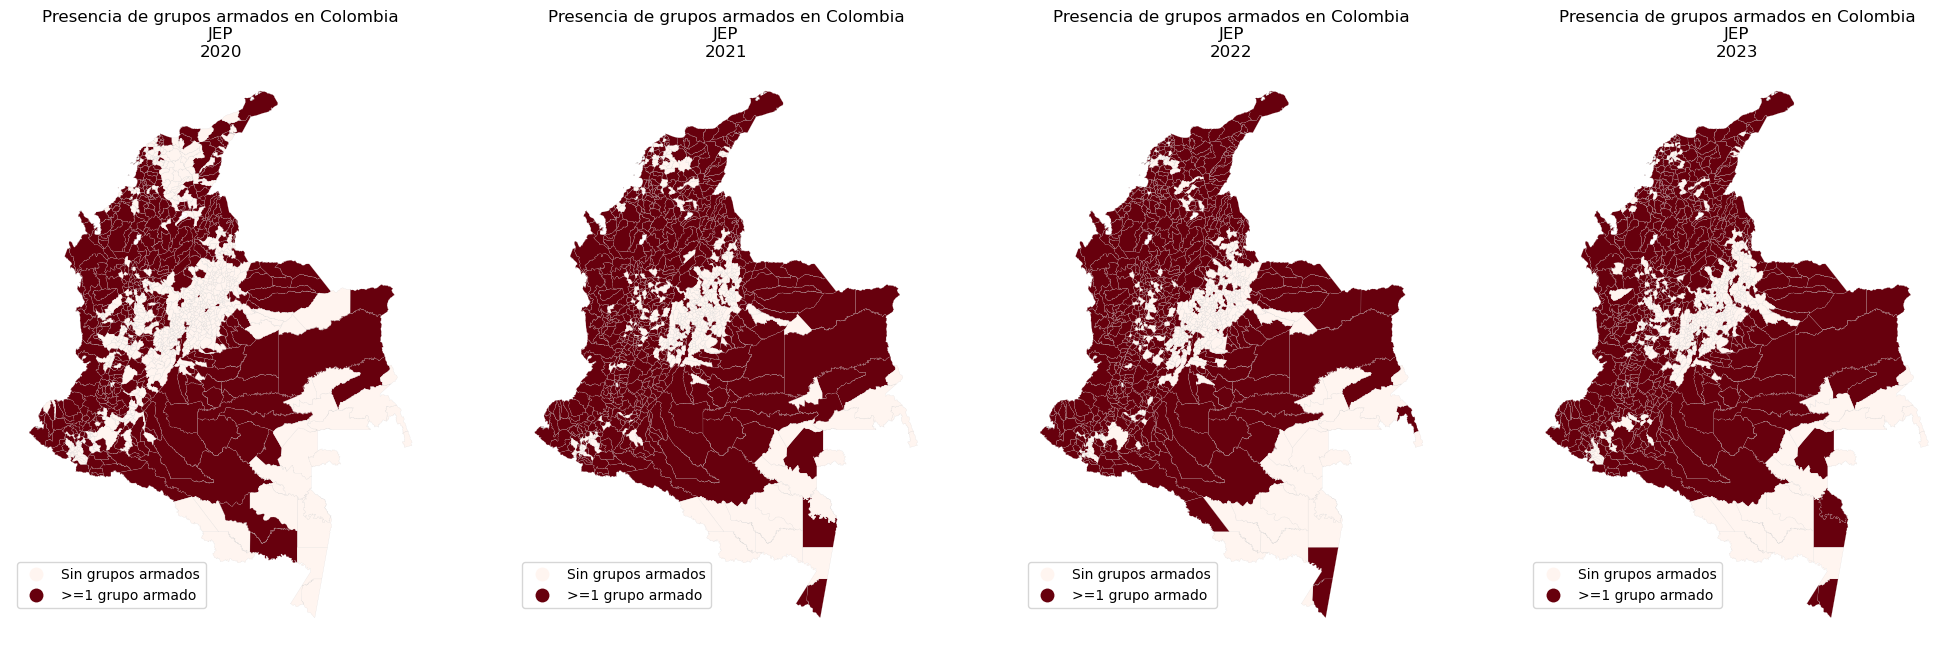
\includegraphics[width=0.8\textwidth]{Seminario de Tesis/Primera presentación/images/image.png}
    \caption{Clasificación binaria de los municipios según la presencia de grupos armados.}
    \label{fig:graph1}
\end{figure}

En cambio, la figura 2 emplea un degradado de color para mostrar cuántos grupos armados hay en cada municipio, desde cero hasta tres al mismo tiempo. Los tonos rojos más intensos indican lugares con varios grupos, lo que refleja una dinámica de violencia más compleja y un mayor riesgo de enfrentamientos. Así, se puede observar la expansión y consolidación de las zonas conflictivas a lo largo del tiempo, evidenciando el incremento de la superposición de grupos en distintas áreas.

\begin{figure}[h!]
    \centering
    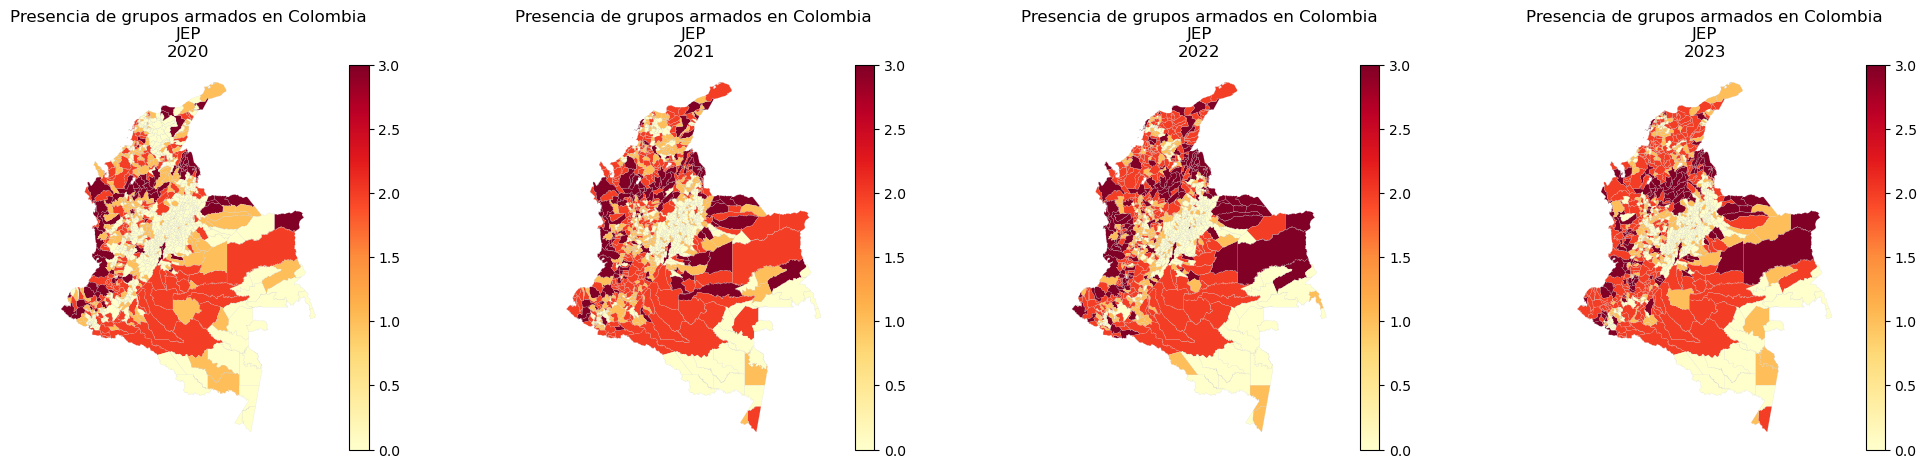
\includegraphics[width=0.8\textwidth]{Seminario de Tesis/Primera presentación/images/image 1.png}
    \caption{Concentración de grupos armados por municipio.}
    \label{fig:graph2}
\end{figure}

Por su parte, la figura 3 muestra la evolución del Índice de Violencia Agregada (IACV) a lo largo del tiempo, comparando los datos de la Fiscalía General de la Nación y del Ministerio de Defensa Nacional. Se observa una tendencia en aumento desde 2020 hasta 2024, aunque con diferencias en la magnitud y variabilidad entre las dos fuentes. Esto sugiere que la expansión de grupos armados en Colombia a través de los años ha venido acompañado de un aumento agregado de la violencia en Colombia.

\begin{figure}[h!]
    \centering
    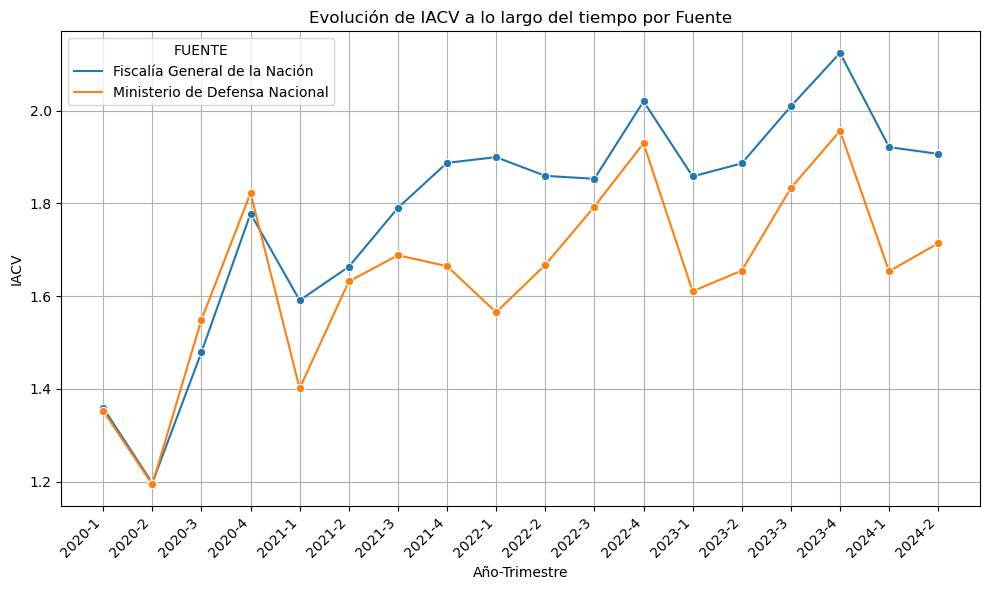
\includegraphics[width=0.8\textwidth]{Seminario de Tesis/Primera presentación/images/image 7.png}
    \caption{Evolución del IACV según los registros de la Fiscalía General de la Nación y el Ministerio de Defensa Nacional.}
    \label{fig:graph3}
\end{figure}

Asimismo, La figura 4 y 5 muestran la Curva de Lorenz del IACV para el año 2019 y 2024 respectivamente. Esta curva sirve para analizar cómo se reparte la violencia entre la población. Cuanto más se aleja la curva de la línea de igualdad perfecta (en rojo), mayor es la concentración en un grupo pequeño de la población. Para 2019, el índice de Gini es de 66\%, lo que indica que la violencia se concentra en pocos municipios. En contraste, para 2024, el índice de Gini sube a 73\%, reflejando que la concentración de la violencia es aún mayor. Así, en conjunto con los gráficos anteriores, se sugiere que este aumento de violencia, que ha sido acompañado de una expansión de grupos criminales en el país, no solo ha aumentado, si no que ha venido aumentando y concentrandose en una menor cantidad de municipios. 

\newpage

\begin{figure}[h1]
    \centering
    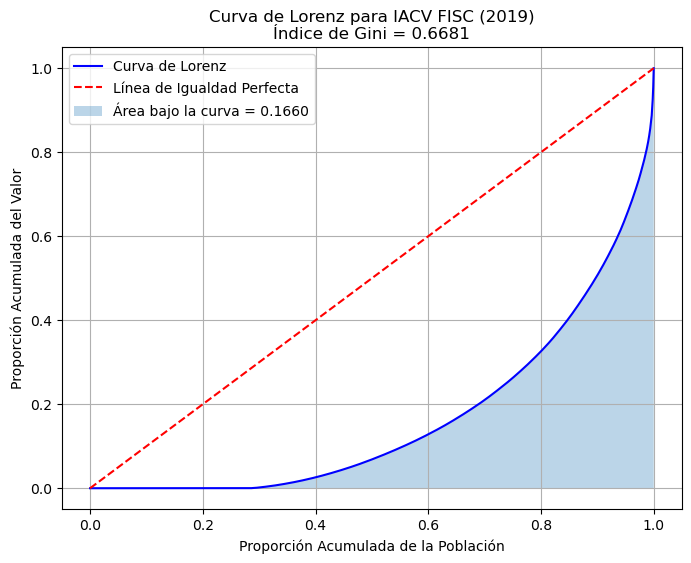
\includegraphics[width=0.7\textwidth]{Seminario de Tesis/Primera presentación/images/image 3.png}
    \caption{Curva de Lorenz del IACV para 2019.}
    \label{fig:graph4}
\end{figure}


\begin{figure}[h!]
    \centering
    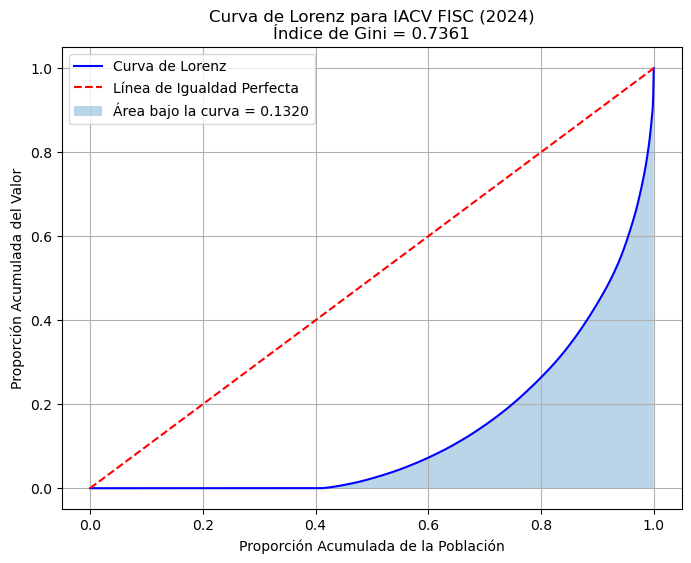
\includegraphics[width=0.7\textwidth]{Seminario de Tesis/Primera presentación/images/image 4.png}
    \caption{Curva de Lorenz del IACV para 2024.}
    \label{fig:graph5}
\end{figure}

\newpage

Finalmente, la figura 6 y 7 muestran la relación entre los quintiles de variables asociadas al desarrollo y bienestar municipal y el valor medio del IACV, junto con sus intervalos de confianza al 95\%. 

Para la figura 6 se utiliza como variable objetivo el índice de necesidades básicas insatisfechas. Se observa un incremento progresivo en el promedio del IACV entre los primeros cuatro quintiles, alcanzando su punto más alto en el cuarto. Por su parte, la figura 7 utiliza como variable objetivo el índice de alfabetización municipal. Se observa una disminución del promedio del IACV a partir del segundo quintil.

Estos resultados indican que la violencia tiende a concentrarse en municipios con niveles de carencias elevados, pero no extremos. En los municipios con las mayores privaciones, quinto quintil en la figura 6 y primer quintil en la figura 7, el IACV presenta una ligera reducción. Asimismo, los intervalos de confianza evidencian la variabilidad de cada grupo y sugieren diferencias estadísticamente significativas.
\newpage
\begin{figure}[h!]
    \centering
    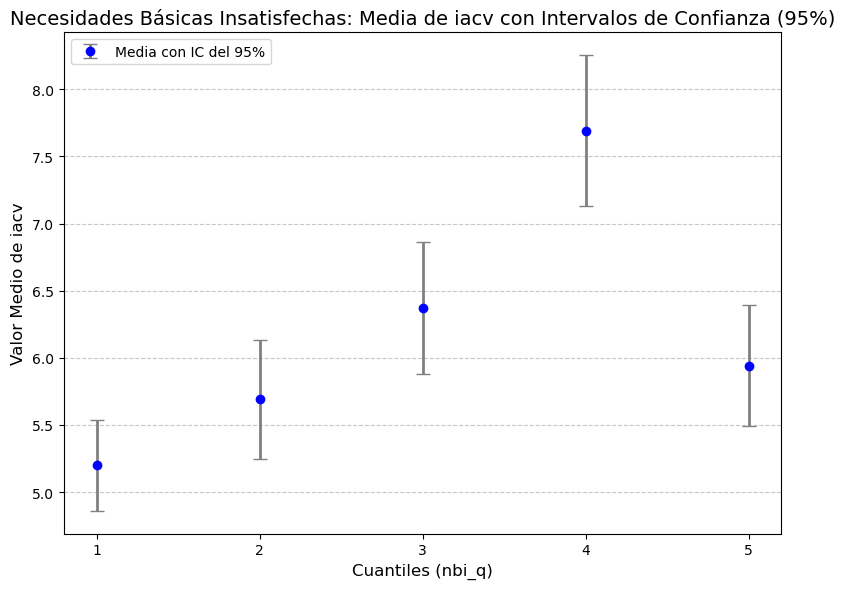
\includegraphics[width=0.7\textwidth]{Seminario de Tesis/Primera presentación/images/output1.png}
    \caption{Necesidades Básicas Insatisfechas vs. IACV con Intervalos de Confianza (95\%).}
    \label{fig:nbivia1}
\end{figure}
\begin{figure}[h!]
    \centering
    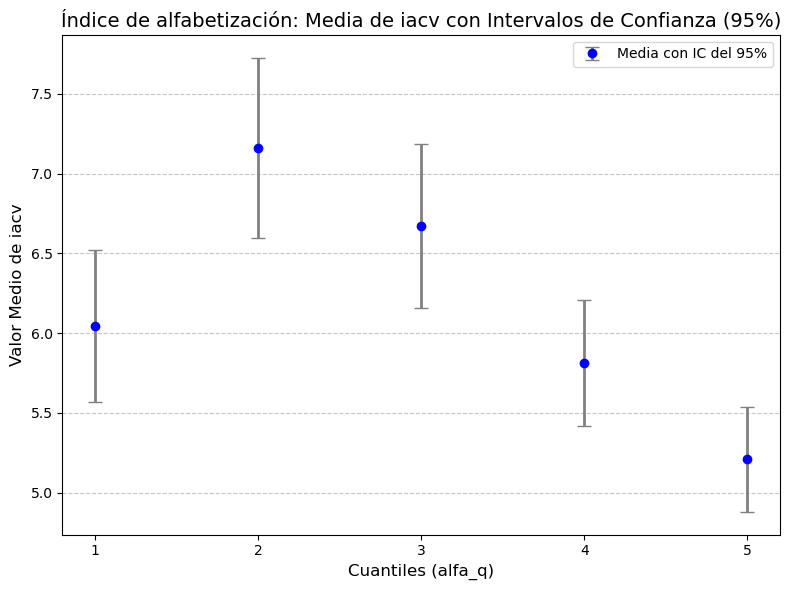
\includegraphics[width=0.7\textwidth]{Seminario de Tesis/Primera presentación/images/output2.png}
    \caption{Alfabetización vs. IACV con Intervalos de Confianza (95\%).}
    \label{fig:nbivia2}
\end{figure}

\newpage
\section{Datos}

\makesection{Datos}
\begin{frame}{Fuentes de Datos}
Los datos de violencia provienen de tres fuentes principales:

\begin{itemize}
    \item \textbf{Fiscalía General de la Nación}: Registros mensuales de \alert{homicidio, extorsión, secuestro, terrorismo y masacres} a nivel municipal, mensual (2014-2024).
    \item \textbf{Ministerio de Defensa Nacional}: Serie histórica de los mismos delitos con \alert{mayor cobertura temporal} a nivel municipal, mensual(1997-2024)%, permitiendo análisis de tendencias a largo plazo. Idea para hacer PCA para los datos antes del corte de la fiscalía
    \item \textbf{Jurisdicción Especial para la Paz (JEP)}: Datos sobre \alert{presencia de grupos armados y eventos violentos} (2017-2024), incluyendo desplazamientos, hostigamientos y paros armados.
\end{itemize}
\end{frame}
\begin{frame}{Fuentes de Datos}

Para analizar la relación entre violencia y factores estructurales, se integran:

\begin{itemize}
    \item \textbf{Panel Municipal del CEDE} (2005-2023): Información demográfica, socioeconómica e institucional, como \alert{pobreza, acceso a servicios y programas para víctimas}.
    \item \textbf{Cultivos ilícitos de coca} (1999-2023, Observatorio de Drogas de Colombia): Financiación de grupos armados y la \alert{dinámica del conflicto}.
    \item \textbf{Luminosidad nocturna (VIIRS Nighttime Light)} (2012-2023): Indicador proxy de \alert{actividad económica local}.
\end{itemize}
\end{frame}

\section{Metodología}
\subsection*{Aprendizaje Automático}
El propósito es estimar, para cada municipio \(m\) y trimestre \(t\), la probabilidad de que ocurra un evento de {violencia atípica}. Formalmente se busca la función
\[
\widehat{P}\bigl(\text{ViolenciaAtípica}_{t,m}=1 \mid \mathbf{X}_{t,m}\bigr),
\]
donde \(\mathbf{X}_{t,m}\) agrupa predictores estructurales y rezagos de violencia.

\subsection*{Clasificación versus regresión}

Se emplea un enfoque de clasificación binaria porque la variable dependiente toma solo dos valores (violencia atípica: sí o no). Los clasificadores permiten estimar probabilidades que se interpretan como riesgos y facilitan la fijación de umbrales operativos. Estos umbrales, a su vez, pueden ajustarse para privilegiar la sensibilidad o la precisión de acuerdo con la capacidad institucional. Además, los resultados son fácilmente integrables en esquemas de priorización de alertas tempranas.

\subsection*{Especificación del modelo}

La probabilidad se representa de forma general como
\[
\text{ViolenciaAtípica}_{t,m}
= f\!\bigl(IACV_{t-1:t-12,m},\, IGC_{t-1:t-4,m},\, IA_{t-1:t-4,m},\, \mathbf{S}_{t,m}\bigr),
\]
donde la función \(f(\cdot)\) se aproxima con dos algoritmos de aprendizaje automático. 
\subsection*{Modelos a utilizar}

El primero es Lasso, una regresión logística con penalización \(L_1\) que selecciona de manera automática los predictores lineales más relevantes (Tibshirani, 1996). Esto modelos lineales mejoran la interpretabilidad del modelo. Así, Lasso simplifica la selección de variables sin comprometer la precisión de las predicciones. Además, es útil para datos con alta dimensionalidad, evitando el sobreajuste mediante la regularización de los coeficientes. Sin embargo, su principal limitación es que sólo captura relaciones lineales entre las variables, lo que podría afectar su desempeño en la predicción de eventos atípicos si existen interacciones no lineales complejas. También requiere una adecuada calibración de sus hiperparámetros, lo que aumenta el costo computacional del entrenamiento.
\\\\
Bosques Aleatorios, propuesto por Breiman (2001), es un modelo basado en la combinación de múltiples {árboles de decisión}, lo que mejora la robustez y precisión del modelo en comparación con un árbol único.
\\\\
Así, es capaz de manejar datos con relaciones no lineales y capturar interacciones complejas entre variables. Además, es resistente al ruido y a la presencia de valores faltantes. Sin embargo, su desventaja principal es la falta de interpretabilidad, ya que la combinación de múltiples árboles dificulta la explicación del proceso de toma de decisiones del modelo. Además, puede ser computacionalmente costoso en grandes volúmenes de datos.

\subsection*{Procedimiento de estimación}

La base de datos se divide en cinco pliegues y se realiza validación cruzada temporal. Dada la naturaleza atípica de estos eventos de violencia, el desbalance se corrige mediante sobremuestreo de la clase minoritaria en el conjunto de entrenamiento. Los hiperparámetros de cada algoritmo se ajustan con validación cruzada, optimizando el F1\-Score. Para evaluar el desempeño se reportan AUC, precisión global, sensibilidad, precisión y tasa de falsos positivos.
\\\\
La probabilidad estimada \(\widehat{P}\bigl(\text{ViolenciaAtípica}_{t,m}=1\bigr)\) se incorpora como puntaje de riesgo en el protocolo del SAT. Los umbrales de decisión se ajustan según las prioridades de política: reducir falsos negativos cuando se teme subestimar eventos críticos o reducir falsos positivos para evitar alertas innecesarias que puedan sobrecargar la capacidad de intervención.

\subsubsection*{Comparación de Modelos y Evaluación de Desempeño}

En el campo del {aprendizaje automático}, es común comparar múltiples modelos para seleccionar el más adecuado según el problema específico. Cada metodología mencionada tiene fortalezas y debilidades, por lo que su desempeño se evaluará utilizando métricas estándar como {precisión, sensibilidad, F1\-Score y AUC}.
\\\\
Para evaluar el desempeño de los modelos en este estudio, se emplearán las siguientes métricas: precisión, sensibilidad, F1\-Score y AUC.
\\\\
\textbf{Precisión: Fiabilidad en la Identificación de Eventos Atípicos}
\\\\
La precisión mide qué proporción de las predicciones positivas realmente corresponden a eventos violentos atípicos. Matemáticamente, se expresa como:

\begin{equation}
\text{Precisión} = \frac{\text{Verdaderos Positivos}}{\text{Verdaderos Positivos} + \text{Falsos Positivos}}
\end{equation}

Desde una perspectiva operativa, una alta precisión significa que el modelo comete pocos errores al identificar eventos atípicos, minimizando el número de falsas alarmas. Esto es fundamental para evitar la sobrecarga de recursos de seguridad, asegurando que los esfuerzos preventivos se concentren en situaciones de riesgo real.
\\\\
\textbf{Sensibilidad: Capacidad de Detectar Eventos Atípicos Reales}
\\\\
La sensibilidad, por otro lado, mide qué proporción de los eventos atípicos reales son correctamente detectados por el modelo. Se define como:

\begin{equation}
\text{Sensibilidad} = \frac{\text{Verdaderos Positivos}}{\text{Verdaderos Positivos} + \text{Falsos Negativos}}
\end{equation}

Una alta sensibilidad es prioritaria en contextos donde el costo de no identificar un evento crítico es mayor que el de generar una falsa alarma. En el caso de la violencia, no detectar un evento atípico a tiempo puede traducirse en pérdida de vidas humanas y en la incapacidad del sistema de alertas para reaccionar adecuadamente ante situaciones de emergencia.
\\\\
\textbf{F1-Score: Equilibrio entre Precisión y Sensibilidad}
\\\\
Dado que existe una disyuntiva entre precisión y sensibilidad, se empleará el F1-Score como métrica de referencia para evaluar el desempeño global del modelo. El F1-Score es la media armónica entre precisión y sensibilidad, proporcionando un balance entre ambos aspectos. Su fórmula es la siguiente:

\begin{equation}
F1 = 2 \times \frac{\text{Precisión} \times \text{Sensibilidad}}{\text{Precisión} + \text{Sensibilidad}}
\end{equation}

Un F1-Score alto indica que el modelo es capaz de detectar la mayoría de los eventos violentos atípicos sin generar un número excesivo de falsas alarmas. En el contexto del presente estudio, esta métrica es clave, ya que permite evaluar si el uso de aprendizaje de máquinas mejora la capacidad predictiva respecto a los métodos tradicionales de alertas tempranas.
\\\\
Además, el uso del F1-Score ayuda a equilibrar dos aspectos fundamentales: la eficiencia en la asignación de recursos y la necesidad de priorizar la protección de la población ante posibles episodios de violencia extrema.
\\\\
\textbf{Área bajo la curva ROC (AUC): capacidad de discriminación independiente del umbral}
\\\\
Esta métrica resume, en un único valor, todas las combinaciones posibles de sensibilidad y tasa de falsos positivos que se obtienen al variar el umbral de clasificación. Al integrar la curva Receiver Operating Characteristic (ROC),
\[
\text{AUC} \;=\; \int_{0}^{1} \!\text{Sensibilidad}(\,\text{Precisión}\,)\;d(\text{Precisión}),
\]
se mide la probabilidad de que el modelo asigne una puntuación de riesgo más alta a un municipio con violencia atípica que a uno sin ella. Por no depender de un umbral específico, la AUC permite comparar modelos en términos de su capacidad inherente para ordenar los casos según su probabilidad subyacente de un evento crítico. En contextos con fuerte desbalance de clases, como el presente, esta característica resulta valiosa porque evita ajustes arbitrarios y se centra en la calidad de la discriminación estadística. Una AUC cercana a 1 indica que el algoritmo clasifica correctamente la mayoría de los pares municipio‐trimestre, mientras que un valor próximo a 0,5 sugiere desempeño no mejor que el azar.
\\\\
En el marco del SAT, la AUC facilita priorizar intervenciones al ofrecer un ranking robusto de municipios según su riesgo estimado, sin necesidad de fijar de antemano el punto de corte que activaría una alerta.

\section{Resultados preliminares}

\begin{table}[h]
\centering
\begin{tabular}{lrr}
\toprule
 & \textbf{Lasso} & \textbf{Bosques Aleatorios} \\
\midrule
AUC             & 0.811 & 0.898 \\
Sensibilidad    & 0.743 & 0.604 \\
Precisión   & 0.707 & 0.997 \\
Precisión global & 0.720 & 0.854 \\
Relación FP/TP  & 0.687 & 0.009 \\
Relación FN/TP  & 0.345 & 0.656 \\
\bottomrule
\end{tabular}
\caption{Desempeño comparado de los modelos (validación cruzada temporal).}
\label{tab:model_comparison}
\end{table}

La Tabla~\ref{tab:model_comparison} presenta los indicadores de desempeño para los dos algoritmos estimados. El modelo Lasso arroja un área bajo la curva ROC (AUC) de 0.81 y combina una sensibilidad de 0.74 con una precisión de 0.71, lo que se traduce en una precisión global de 0.72. Estos valores sugieren que, bajo relaciones lineales, el conjunto de predictores históricos y estructurales ofrece una capacidad moderada para identificar brotes de violencia atípica.
\\\\
El {Bosques Aleatorios}, por su parte, eleva la AUC a 0.90 y la precisión global a 0.85. La precisión alcanza 0.997, lo cual reduce de forma drástica la proporción de falsas alarmas (FP/TP = 0.009). Sin embargo, la sensibilidad desciende a 0.60 y, en consecuencia, la relación de falsos negativos aumenta. En términos operativos, el modelo basado en árboles discrimina mejor los municipios verdaderamente críticos, aunque pasa por alto algunos eventos menos evidentes.
\\\\
La ganancia en precisión refleja la capacidad del {Bosques Aleatorios} para capturar interacciones no lineales entre los índices de violencia, los factores estructurales y la dinámica reciente del conflicto. La menor sensibilidad sugiere que, si la prioridad institucional es evitar omisiones, podría ser necesario ajustar el umbral de decisión o incorporar técnicas complementarias que eleven la detección de casos positivos.
\\\\
En síntesis, los resultados preliminares indican que el {Bosques Aleatorios} supera al Lasso en la mayoría de las métricas relevantes, especialmente en la reducción de alertas erróneas. Esta mejora ofrece un argumento sólido para integrar el puntaje de riesgo del modelo en el protocolo del SAT, siempre que se calibren los umbrales de alerta de acuerdo con los objetivos de política pública y la capacidad de respuesta disponible.

\section{Conclusiones y líneas de trabajo futuro}

La evidencia preliminar muestra que los modelos de aprendizaje automático pueden complementar el {Sistema de Alertas Tempranas} (SAT) al estimar con mayor precisión la probabilidad de violencia atípica a nivel municipal. Entre los dos algoritmos evaluados, el {Bosques Aleatorios} destaca por un área bajo la curva ROC de 0.90 y una reducción de 98\,\% en la proporción de falsas alarmas respecto al Lasso. Estos resultados sugieren que estimaciones no lineales y pronósticos permiten identificar con mayor certeza los municipios más expuestos a eventos atípicos, lo cual puede optimizar la asignación de recursos preventivos.
\\\\
Al mismo tiempo, la menor sensibilidad del {Bosques Aleatorios} advierte sobre el riesgo de omitir algunos eventos. Otro desafío consiste en traducir las probabilidades en protocolos claros para el personal del SAT, de modo que la información sea accionable y se evite la sobrecarga de alertas.
\\\\
Las líneas de trabajo futuro se orientan en tres direcciones. En primer lugar, se planea evaluar algoritmos adicionales como XGBoost y LSTM para contrastar la robustez de los hallazgos y, en particular, mejorar la sensibilidad sin sacrificar especificidad. En segundo lugar, se propone incorporar fuentes de datos textuales, provenientes de los informes del SAT, para poder complmentar las señales tempranas sobre tensiones locales. 
\\\\
Finalmente, este estudio aporta un marco reproducible que combina aprendizaje automático y análisis cualitativo para fortalecer las alertas tempranas de violencia; las extensiones previstas buscan consolidar su utilidad práctica y ampliar la capacidad de la Defensoría del Pueblo para proteger a las poblaciones en riesgo.






\newpage
%\bibliographystyle{apalike}
%\bibliography{referencias}
\section*{Referencias}

\begin{itemize}
    \item Banco Interamericano de Desarrollo. (2017). \textit{Informe sobre el costo de la criminalidad en América Latina}. Banco Interamericano de Desarrollo.
    
    \item Barreras, F., Díaz, C., Riascos, Á. J., \& Ribero, M. (2016). \textit{Una comparación de diferentes modelos para la predicción del crimen en Bogotá}. Universidad de los Andes, CESED.
    
    \item Bazzi, S., Blair, R. A., Blattman, C., Dube, O., Gudgeon, M., \& Peck, R. (2019). \textit{The Promise and Pitfalls of Conflict Prediction: Evidence from Colombia and Indonesia} (NBER Working Paper 25980). National Bureau of Economic Research.
    
    \item D'Orazio, V. (2023). \textit{Probabilistic Conflict Forecasting with Automated Machine Learning}. Contribution to ViEWS Prediction Challenge 2023/24, West Virginia University. 
    
    \item Feldmann, A. E., \& Hinojosa, V. M. (2009). Terrorism in Colombia: Logic and Sources of a Multidimensional and Ubiquitous Phenomenon. \textit{Terrorism and Political Violence}, \textit{21}(1), 42--61.
    
    \item Giraldo Alegría, S. A., Ordoñez Palacios, L. E., Bucheli, V., \& Ordoñez, H. (2020). Modelo de redes neuronales para predecir la tendencia de víctimas de secuestro en Colombia. \textit{Investigación e Innovación en Ingenierías}, \textit{8}(3), 38--49. \url{https://doi.org/10.17081/invinno.8.3.4702}
    
    \item Hochreiter, S., \& Schmidhuber, J. (1997). Long short-term memory. \textit{Neural Computation}, \textit{9}(8), 1735--1780.
    
    \item Levitt, S., \& Rubio, M. (2000). \textit{Understanding Crime in Colombia and What Can Be Done About It}. Documento de trabajo, Universidad de Chicago/Fedesarrollo.
    
    \item Mohler, G., Short, M. B., Brantingham, P. J., Schoenberg, F. P., \& Tita, G. (2011). Self-Exciting Point Process Modeling of Crime. \textit{Proceedings of the National Academy of Sciences}, \textit{108}(19), 7743--7748. \url{https://doi.org/10.1073/pnas.1015346108}
    
    \item Musumba, M., Fatema, N., \& Kibriya, S. (2021). Prevention Is Better Than Cure: Machine Learning Approach to Conflict Prediction in Sub-Saharan Africa. \textit{Sustainability}, \textit{13}(13), 7366. \url{https://doi.org/10.3390/su13137366}
    
    \item Ordoñez Eraso, H. A., Pardo Calvache, C. J., \& Cobos Lozada, C. A. (2020). Detection of Homicide Trends in Colombia Using Machine Learning. \textit{Revista Facultad de Ingeniería (University of Antioquia)}, \textit{29}(54), e105.
    
    \item Radford, B. J. (2022). High resolution conflict forecasting with spatial convolutions and long short-term memory. \textit{International Interactions}, \textit{48}(4), 739--758. \url{https://doi.org/10.1080/03050629.2022.2031182}
    
    \item Riascos, Á. J., \& Vargas, J. F. (2011). \textit{Violence and Growth in Colombia: A Review of the Quantitative Literature} (Documentos de Trabajo No. 8806). Universidad del Rosario.
    
    \item Rod, E. G., Hegre, H., \& Leis, M. R. (2023). Predicting armed conflict using protest data. \textit{Journal of Peace Research}. \url{https://doi.org/10.1177/00223433231186452}
    
    \item Rojas, J., \& Grautoff, C. (2023). \textit{Predicción de las masacres en Colombia empleando inteligencia artificial}. Universidad de los Andes, Working Paper.
    
    \item Rubio, M. (1999). \textit{Crimen e impunidad: Precisiones sobre la violencia}. Documento CEDE, Universidad de los Andes.
    
    \item Rubio, M. (2000). \textit{La Violencia en Colombia: Precisiones económicas}. Inter-American Development Bank.
    
    \item Rubio, M. (2003). \textit{El rapto de la pesca milagrosa: breve historia del secuestro en Colombia} (Documento de trabajo No. 2003-36). CEDE, Universidad de los Andes.
    
    \item Sánchez, F., \& Núñez, J. (2001). \textit{Determinantes del crimen violento en un país altamente violento: El caso de Colombia}. CEDE, Universidad de los Andes.
    
    \item Sánchez, F., \& Chacón, M. (2005). Conflicto, Estado y descentralización: Del progreso social a la disputa armada por el control local, 1974–2002. \textit{Documentos CIDER, Universidad de los Andes/LSE}.
    
    \item Urcuqui, C., Moreno, J. S., Montenegro, C., Riascos, Á., \& Dulce, M. (2020). Accuracy and Fairness in a Conditional Generative Adversarial Model of Crime Prediction. \textit{2020 IEEE International Conference on Systems, Man, and Cybernetics (SMC)}, 1631--1636. \url{https://doi.org/10.1109/SMC42975.2020.9283477}
    
    \item Zou, H., \& Hastie, T. (2005). Regularization and variable selection via the elastic net. \textit{Journal of the Royal Statistical Society: Series B (Statistical Methodology)}, \textit{67}(2), 301--320.
    
    \item Breiman, L. (2001). Random forests. \textit{Machine Learning}, \textit{45}(1), 5--32.
    
    \item Chen, T., \& Guestrin, C. (2016). XGBoost: A scalable tree boosting system. In \textit{Proceedings of the 22nd ACM SIGKDD International Conference on Knowledge Discovery and Data Mining} (pp. 785--794).
\end{itemize}
\end{document}
